\section{How to estimate time-varying coefficient $\beta$}

%Reference:
%\cite{chu2016feature}

%FEATURE SCREENING FOR TIME-VARYING COEFFICIENT MODELS WITH ULTRAHIGH DIMENSIONAL LONGITUDINAL DATA

\subsection{Observations in ADNI1}

There are \underline{819 patients} and \underline{5122} longitudinal observations when I use \underline{MMSE} as response variable.


\begin{table}[h]
    \centering
    \begin{tabular}{c|c}
    \hline
       value  & n \\ \hline
       1  & 34 \\
       2  & 44 \\
       3  & 54 \\
       4  & 64 \\
       5  & 34 \\
       6  & 74 \\
     \hline
     \end{tabular}\label{tab:my_label}
\end{table}




\subsection{How to Set Time Points}


\begin{itemize}
     
\item Treat the smallest age of patients in ADNI1 as 0.

\item Treat the age at baseline of each patient as its original age, then add the \underline{date difference over 365} to the original age as its new age.
\end{itemize}




\subsection{Time-Varying Coefficient Plots for 2 SNPs}

Refer to Chu's \citet{chu2016feature}idea, we generate our time-varying coefficient plot.

\begin{figure}[H]
\centering  

\subfigure[rs7252864]{
\begin{minipage}[b]{\textwidth}
\label{Fig.1.41}
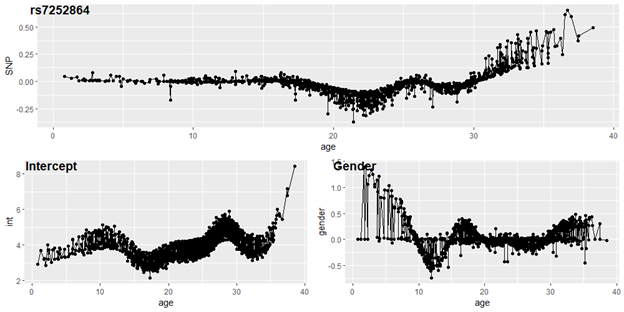
\includegraphics[width=0.8\textwidth]{Figures/1.4-1.png}
\end{minipage}}

\subfigure[APOE4]{
\begin{minipage}[b]{\textwidth}
\label{Fig.1.42}
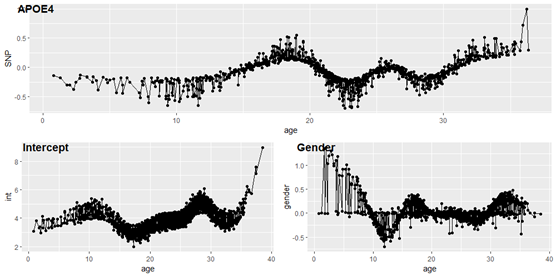
\includegraphics[width=0.8\textwidth]{Figures/1.4-2.png}
\end{minipage}}
%\caption{Main name}
\label{Fig.1.4}
\end{figure}


